% Options for packages loaded elsewhere
\PassOptionsToPackage{unicode}{hyperref}
\PassOptionsToPackage{hyphens}{url}
%
\documentclass[
]{article}
\usepackage{amsmath,amssymb}
\usepackage{iftex}
\ifPDFTeX
  \usepackage[T1]{fontenc}
  \usepackage[utf8]{inputenc}
  \usepackage{textcomp} % provide euro and other symbols
\else % if luatex or xetex
  \usepackage{unicode-math} % this also loads fontspec
  \defaultfontfeatures{Scale=MatchLowercase}
  \defaultfontfeatures[\rmfamily]{Ligatures=TeX,Scale=1}
\fi
\usepackage{lmodern}
\ifPDFTeX\else
  % xetex/luatex font selection
\fi
% Use upquote if available, for straight quotes in verbatim environments
\IfFileExists{upquote.sty}{\usepackage{upquote}}{}
\IfFileExists{microtype.sty}{% use microtype if available
  \usepackage[]{microtype}
  \UseMicrotypeSet[protrusion]{basicmath} % disable protrusion for tt fonts
}{}
\makeatletter
\@ifundefined{KOMAClassName}{% if non-KOMA class
  \IfFileExists{parskip.sty}{%
    \usepackage{parskip}
  }{% else
    \setlength{\parindent}{0pt}
    \setlength{\parskip}{6pt plus 2pt minus 1pt}}
}{% if KOMA class
  \KOMAoptions{parskip=half}}
\makeatother
\usepackage{xcolor}
\usepackage[margin=1in]{geometry}
\usepackage{longtable,booktabs,array}
\usepackage{calc} % for calculating minipage widths
% Correct order of tables after \paragraph or \subparagraph
\usepackage{etoolbox}
\makeatletter
\patchcmd\longtable{\par}{\if@noskipsec\mbox{}\fi\par}{}{}
\makeatother
% Allow footnotes in longtable head/foot
\IfFileExists{footnotehyper.sty}{\usepackage{footnotehyper}}{\usepackage{footnote}}
\makesavenoteenv{longtable}
\usepackage{graphicx}
\makeatletter
\def\maxwidth{\ifdim\Gin@nat@width>\linewidth\linewidth\else\Gin@nat@width\fi}
\def\maxheight{\ifdim\Gin@nat@height>\textheight\textheight\else\Gin@nat@height\fi}
\makeatother
% Scale images if necessary, so that they will not overflow the page
% margins by default, and it is still possible to overwrite the defaults
% using explicit options in \includegraphics[width, height, ...]{}
\setkeys{Gin}{width=\maxwidth,height=\maxheight,keepaspectratio}
% Set default figure placement to htbp
\makeatletter
\def\fps@figure{htbp}
\makeatother
\setlength{\emergencystretch}{3em} % prevent overfull lines
\providecommand{\tightlist}{%
  \setlength{\itemsep}{0pt}\setlength{\parskip}{0pt}}
\setcounter{secnumdepth}{5}
\ifLuaTeX
  \usepackage{selnolig}  % disable illegal ligatures
\fi
\usepackage{bookmark}
\IfFileExists{xurl.sty}{\usepackage{xurl}}{} % add URL line breaks if available
\urlstyle{same}
\hypersetup{
  pdftitle={Review1\_NewFigs},
  pdfauthor={Sophie Wulfing},
  hidelinks,
  pdfcreator={LaTeX via pandoc}}

\title{Review1\_NewFigs}
\author{Sophie Wulfing}
\date{2024-06-27}

\begin{document}
\maketitle

\begin{longtable}[]{@{}llll@{}}
\caption{\label{tab:DefaultParamTable}(ref:defaultparamtable) \label{DefaultParamTable}}\tabularnewline
\toprule\noalign{}
Parameter & Population 1 & Population 2 & Definition \\
\midrule\noalign{}
\endfirsthead
\toprule\noalign{}
Parameter & Population 1 & Population 2 & Definition \\
\midrule\noalign{}
\endhead
\bottomrule\noalign{}
\endlastfoot
r & 0.16 & 0.16 & Fish net growth \\
s & 0.8 & 0.8 & Supply and demand \\
h & 0.25 & 0.25 & Harvesting efficiency \\
k & 0.17 & 0.17 & Rate of sampling opinions or social interaction \\
\(\omega\) & 1.44 & 1.44 & Conservation cost \\
c & 0.5 & 0.5 & Rarity valuation \\
d & 0.3 & 0.3 & Strength of social influence (within population) \\
m & 0.01 & 0.01 & Fish movement (from opposite patch) \\
\(\rho\) & 0.01 & 0.01 & Strength of social influence (from opposite population) \\
\end{longtable}

\section{NEW FIG}\label{new-fig}

Figure \ref{MovementBothRho} is going to be a new addition to the manuscript. This is basically showing that increases in rho delays decision making but a high increase will eventually lead to collapse. This can also relate to reviewers point about delayed decision making and timescales of conservation decisions



\begin{figure}
\centering
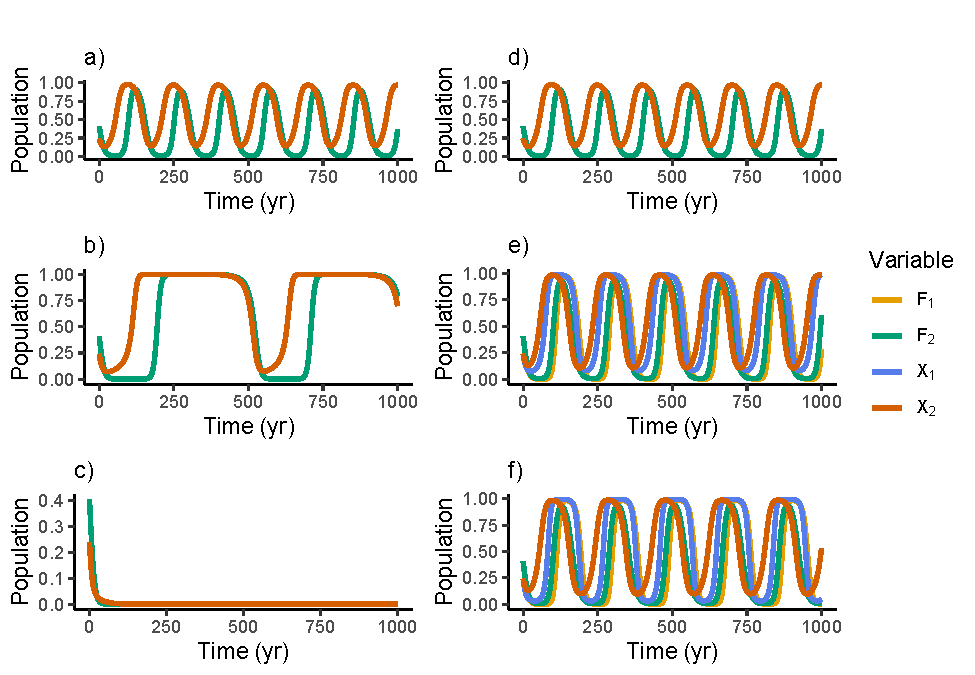
\includegraphics{Review1_NewFigsNotes_files/figure-latex/MovementBothRho-1.pdf}
\caption{\label{fig:MovementBothRho}In graphs a), b), and c), both \(\rho_1\) and \(\rho_2\) were set to 0.01, 0.25, and 0.5, respectively. The corresponding graphs show the dynamics of these models with the new parameterizations. d), e), and f) show the changes in model dynamics when \(\rho_2\) is held at 0.01 and only \(\rho_1\), the social influence of human population 1 onto human population 2 is increased by 0.01, 0.25, and 0.5, respectively. \label{MovementBothRho}}
\end{figure}

\section{REPLACEMENT FIG}\label{replacement-fig}

Make sure you change params on this document code

You could also possibly put the BothRhos document into appendix to show delayed decision making

\begin{longtable}[]{@{}llll@{}}
\caption{\label{tab:NewParamTable}(ref:newparamtable) \label{NewParamTable}}\tabularnewline
\toprule\noalign{}
Parameter & Population 1 & Population 2 & Definition \\
\midrule\noalign{}
\endfirsthead
\toprule\noalign{}
Parameter & Population 1 & Population 2 & Definition \\
\midrule\noalign{}
\endhead
\bottomrule\noalign{}
\endlastfoot
r & 0.4 & 0.35 & Fish net growth \\
s & 0.8 & 0.8 & Supply and demand \\
h & 0.25 & 0.5 & Harvesting efficiency \\
k & 1.014 & 1.014 & Rate of sampling opinions or social interaction \\
\(\omega\) & 0.2 & 0.35 & Conservation cost \\
c & 1.5 & 1.5 & Rarity valuation \\
d & 0.5 & 0.5 & Strength of social influence (within population) \\
m & 0.2 & 0.2 & Fish movement (from opposite patch) \\
\(\rho\) & 0.5 & 0.1 & Strength of social influence (from opposite population) \\
\end{longtable}



\begin{figure}
\centering
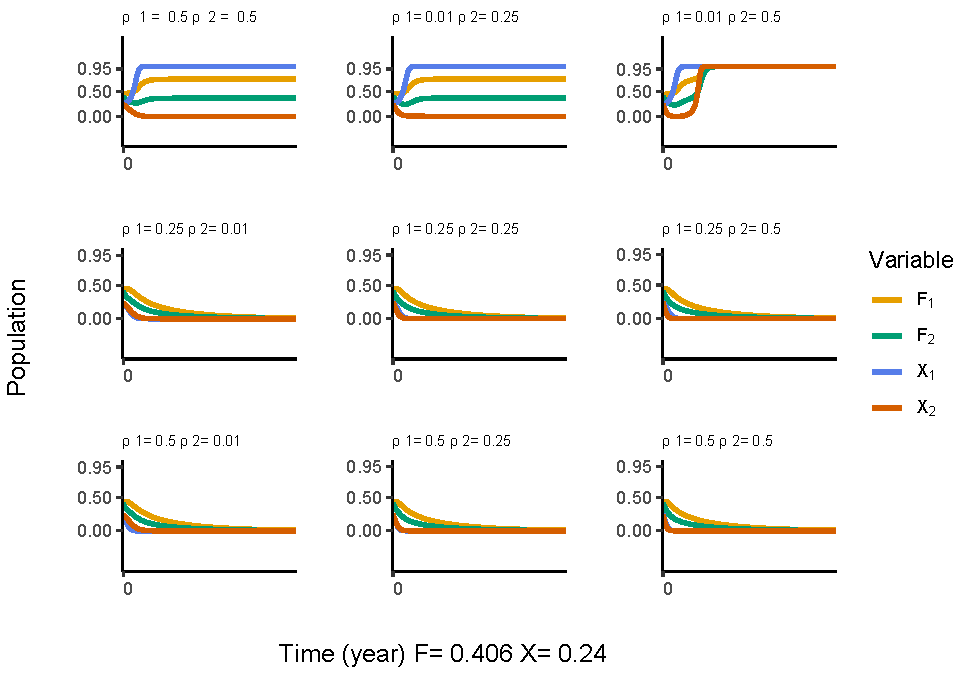
\includegraphics{Review1_NewFigsNotes_files/figure-latex/influenceAsymGraph-1.pdf}
\caption{\label{fig:influenceAsymGraph}The difference in increasing outside social pressure on population 1 (the \(\rho_1\) parameter is increased down the columns of graphs) versus increasing social pressure from population 1 onto population 2 (the \(\rho_2\) parameter is increased across rows of graphs) which compares self-pressure to pressuring the other gropu. \label{influenceAsymGraph}}
\end{figure}





\begin{figure}
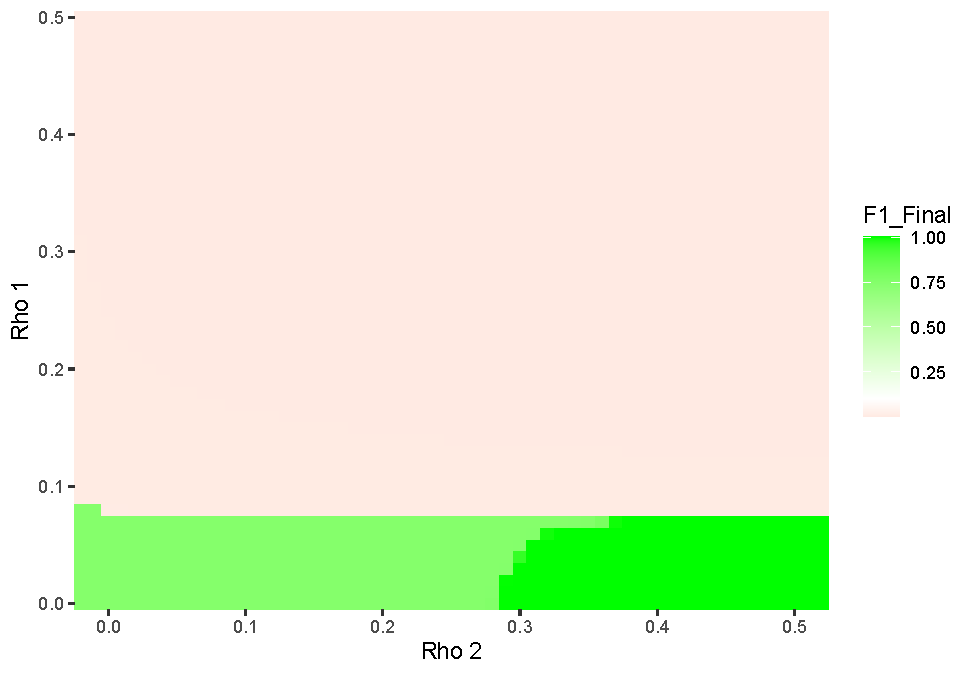
\includegraphics[width=0.5\linewidth]{Review1_NewFigsNotes_files/figure-latex/TwoGraphs-1} 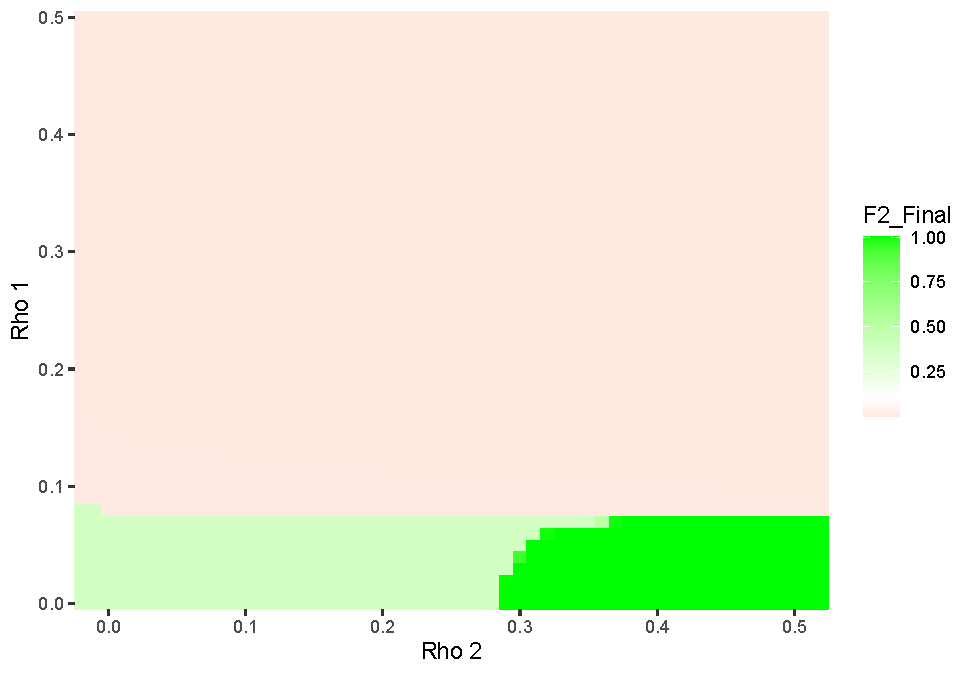
\includegraphics[width=0.5\linewidth]{Review1_NewFigsNotes_files/figure-latex/TwoGraphs-2} \caption{The effect of changing rho 1 and rho 2 on final dynamics of F1 (a) and F2 (b) using parameters from Table 2. Data was run for 200 years \label{TwoGraphs}}\label{fig:TwoGraphs}
\end{figure}

\end{document}
